\begin{frame}{Модели и численные схемы}
\begin{itemize}
  \item Физические уравнения модели прогноза погоды WRF v.3 \cite{wrf:arw}
  \item Численные схемы адвекции
\begin{itemize}
  \item Ориентированы на пассивные примеси
  \item Сохранение массы
  \item Эйлеровы модели
    \begin{itemize}
    \item Ограничения на временной шаг
    \end{itemize}
  \item Полу-Лагранжевые модели:
    \begin{itemize}
    \item Большие временные шаги без потери стабильности
    \item Порядок точности
    \item Сохранение массы/положительно-определенность
    \item Overshooting/undershooting
  \end{itemize}
\end{itemize}

\end{itemize}



\begin{figure}
\centering
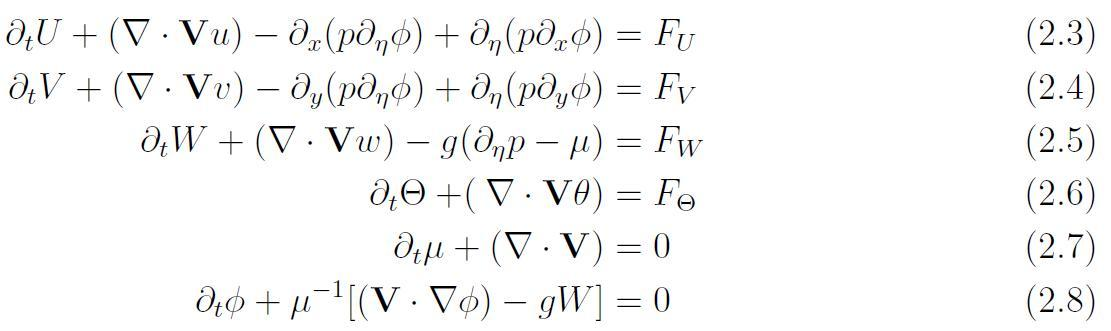
\includegraphics[height=1in, width=3in]{artwork/images/wrf_governing_equations}
\label{fig:wrf-equations}
\end{figure}

\end{frame}



\begin{frame}{Характерные особенности MPDATA}
Специально разработана под метеорологические нужды:
\begin{itemize}
  \item Положительная определенность
  \item Сохранение массы
  \item Вычислительная простота, сравнимая с донорной схемой
\end{itemize}
\end{frame}


\begin{frame}{Расширения MPDATA}
Численная модель вычислений MPDATA хорошо теоретически проработана и включает следующие расширения \cite{smolar:mpdata-solver}:
\begin{itemize}
  \item Возможность увеличить пространственную точность до третьего порядка, временную точность до пятого
  \item Возможность эмпирической подстройки для увеличения точности без увеличения вычислительной сложности
  \item Физическая диффузия в составе адвективного потока
  \item Траспорт скалярного поля с переменным знаком
  \item Моделирование дивергентных полей
\end{itemize}
\end{frame}

\begin{frame}{Почему MPDATA?}
\begin{itemize}
\item Численная модель вычислений MPDATA потенциально может быть оптимизирована под CUDA:
\begin{itemize}
  \item Соотношение доступов в память к вычислениям
  \item Явная модель вычислений
\end{itemize}
  \item Является частью численных гидродинамических моделей погоды EULAG и NH3D
\end{itemize}
\end{frame}


